\documentclass[conference]{IEEEtran}
\usepackage{graphicx}
\usepackage{booktabs}
\usepackage{amsmath,amssymb}
\usepackage{url}
\usepackage{array}
\usepackage[T1]{fontenc}

\graphicspath{{figs/}}
\newcommand{\ms}{\,ms}
\newcommand{\fn}[1]{\textsf{#1}}

\begin{document}

\title{Will the Brake Arrive in Time? Attack-Aware Worst-Case Latency Bounds and Defence Assessment for CAN-Based Software-Defined Vehicles}

\author{\IEEEauthorblockN{Anonymous Authors (double-blind submission)}
\IEEEauthorblockA{Affiliation withheld}}

\maketitle

\begin{abstract}
Software-defined vehicles move safety functions onto shared networks, so an attacker who only delays or distorts messages can consume the time budget a function needs. Intrusion-detection scores such as recall and F1 do not say whether protection arrives before the \emph{point of no return}, the last instant at which a collision can still be avoided. We study this for an emergency-braking chain on classical CAN. We (i)~derive an attack-aware worst-case bound on the obstacle-to-brake latency from CAN response-time analysis with bounded-budget attacker streams, and compare it with an exact closed-form point of no return; (ii)~assess defences (radar failover, a gateway guard, message authentication with a fail-safe watchdog) by the share of the attack space that still causes a collision, using one fresh scenario per sampled attack; and (iii)~check the model against real traffic (two vehicles), a physics simulator and an embedded C port. The bound was never violated in more than 44{,}000 simulated runs nor by 350 adversarial searches, which also exposed flaws in earlier versions. With all defences, a dual-sensor forgery still causes a collision in 4.3\% of the attack space, and a flood from a node already on the safety bus (about 25\%) and an attacker holding the signing key (about 43\%) are not stopped at all. A best detector flags only 63\% of attack-induced hazards in time although its F1 is 0.95. The evidence is an emulation with assumed timings; we state what the real-data checks do and do not support, including two negative results.
\end{abstract}

\begin{IEEEkeywords}
software-defined vehicle, CAN bus, intrusion detection, worst-case latency, point of no return, message authentication
\end{IEEEkeywords}

\section{Introduction}
A modern vehicle runs safety functions such as automatic emergency braking across several electronic control units (ECUs) that exchange messages on shared buses. Each function has a latency budget: if the chain from sensor to actuator takes too long, braking starts too late. An attacker does not need to break the function itself. Flooding the bus, delaying a gateway, or forging a sensor distance can use up the budget, and in software-defined vehicles, where functions and updates are increasingly decoupled from hardware, the number of places from which this can be done grows.

The usual way to judge an intrusion detection system (IDS) is by recall, precision or F1 on labelled traffic~\cite{stachowski2019}. These numbers say little about whether a detection is \emph{useful}: an alarm that comes after the vehicle can no longer stop is worth nothing for that event. The cyber-physical-systems literature has a name for the missing quantity, the \emph{detection deadline}: the time before which an attack must be detected for the system to remain safe~\cite{akowuah2021,zhang2020}. We adopt this notion; we do not claim it as ours.

This paper applies it to bus-level attacks on a CAN-based braking chain, where timing is decided by arbitration and queueing and not only by the controller. We ask three questions. \textbf{Q1:} do standard detection scores reflect protection in time? \textbf{Q2:} can the worst-case time to brake under attack be bounded analytically, so that a given attack instance can be \emph{proven} harmless for every random draw? \textbf{Q3:} which defences close which attack classes, and what remains?

\textbf{Contributions.}
\begin{enumerate}
\item An attack-aware upper bound on obstacle-to-brake latency, built from non-preemptive fixed-priority CAN response-time analysis~\cite{davis2007} with frame-budgeted attacker streams, a busy-period argument for floods, and compute-time worst cases, compared with an exact closed-form point of no return. We validate it by simulation and by adversarial search, and report the flaws that the search found in earlier versions.
\item A defence assessment that reports, per attack variant and defence configuration, the share of the attack space that still causes a collision (Wilson intervals), with one freshly drawn scenario per sampled attack. This design matters: reusing a few scenarios understated the residual risk of one configuration by a factor of four, which we document as an erratum.
\item Checks against real data (ROAD, HCRL), a physics simulator (CARLA) and an embedded C implementation, with the results that did \emph{not} support the model stated plainly.
\item An open, reproducible artifact whose cloud run reproduces the local tables.
\end{enumerate}
To our knowledge, among the work we reviewed, none combines a CAN response-time bound with attacker models and an exact point of no return in this way. The contribution is applied and incremental, and Section~\ref{sec:limits} states the limits.

\section{Related Work}
\textbf{Detection deadlines.} Akowuah and Kong define the detection deadline for sensor attacks in autonomous cyber-physical systems and adapt the detector window to it~\cite{akowuah2021,akowuah2023}; Zhang et al.\ estimate such deadlines by reachability and add recovery~\cite{zhang2020}. These works address sensor and controller dynamics. We work one level lower, on message timing on a shared bus, and replace reachability by a closed-form braking model whose point of no return is exact. A recent indicator study uses the point of no return for rear-end conflicts observed in video~\cite{ponr2026}.

\textbf{CAN timing analysis.} Response-time analysis for non-preemptive fixed-priority scheduling, as revised by Davis et al.~\cite{davis2007}, bounds the delay of a CAN frame given the periodic traffic. We extend it with attacker streams that have a frame budget and release jitter, and with a backlog argument for floods whose queue outlives the flood.

\textbf{Attacks on braking functions.} Berdich and Groza model replay, denial-of-service and fuzzing attacks on adaptive cruise control and emergency braking in Simulink, each succeeding with a fixed probability, and study countermeasures~\cite{berdich2024}. We instead emulate the bus mechanisms (arbitration, queueing, gateway tampering) so that success is a consequence of timing. Zhang's dissertation secures CAN against spoofing, replay and flooding~\cite{zhangthesis}; our defences are deliberately simple and our interest is what each one provably leaves open.

\textbf{IDS assessment.} The NHTSA assessment method~\cite{stachowski2019} lists detection speed among its criteria but scores rates; we add whether the alarm comes before the point of no return.

\textbf{Data.} ROAD provides real masquerade attacks verified on a vehicle~\cite{road}; the HCRL Car-Hacking set provides flooding, fuzzing and spoofing captures from a second vehicle~\cite{hcrl}; CARLA is a widely used simulator~\cite{carla}. We use them as checks, not as training sets.

\section{System and Threat Model}
\begin{figure}[t]
\centering
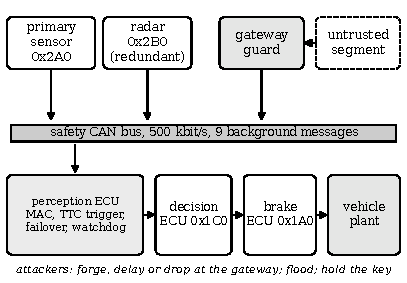
\includegraphics[width=\columnwidth]{fig_arch.pdf}
\caption{The emulated system. Sensor and radar frames reach the perception ECU over a 500\,kbit/s CAN bus shared with nine periodic background messages (13\% of the bus capacity); the untrusted segment (OBD-II, infotainment) is separated by a gateway guard.}
\label{fig:arch}
\end{figure}

\textbf{Emulated chain.} Fig.~\ref{fig:arch} shows the system. A discrete-event emulator runs in integer microseconds. Frames use classical CAN (11-bit IDs, worst-case bit stuffing), and the lowest ID wins arbitration. The brake chain is sensor (ID 0x2A0, 10\,ms period) $\rightarrow$ perception (25\,ms mean compute) $\rightarrow$ decision (0x1C0, 15\,ms) $\rightarrow$ brake command (0x1A0) $\rightarrow$ actuator (25\,ms). Compute times are scaled by CPU load and carry log-normal jitter ($\sigma=0.15$). An optional independent radar (0x2B0) provides a second distance channel. Perception raises a hazard when the reported time-to-collision is at most 2\,s. All timings are assumptions; Section~\ref{sec:eval} varies them.

\textbf{Plant and point of no return.} The vehicle holds its speed until the brake takes effect, then brake force ramps linearly to $\mu g$ over a ramp time and stays constant. With latency $L$, travelled distance is $v_0L$ plus the braking distance (ramp, then constant deceleration). The \emph{point of no return} is the largest latency $L^\ast$ with $v_0L^\ast+s_{\text{brake}}\le d_0$. It is exact for the model. A collision is avoidable iff the actual latency is at most $L^\ast$.

\textbf{Attackers.} Table~\ref{tab:attacks} lists nine families and a phantom-obstacle availability attack. Each declares the access it needs (a compromised node, or a gateway or ECU between a sender and the bus) and parameter ranges. Two further variants make the residual explicit: a flood sent from a node \emph{on} the safety bus (so a gateway cannot see it), and forging attackers that \emph{hold the signing key}. Times are relative to the moment the obstacle becomes a threat, and an attack may start before it.

\begin{table}[t]
\caption{Attack families (all on the emulated bus).}
\label{tab:attacks}
\centering
\footnotesize
\begin{tabular}{@{}p{0.34\columnwidth}p{0.6\columnwidth}@{}}
\toprule
Family & Effect \\
\midrule
DoS flood, priority abuse & back-to-back frames with a high-priority ID \\
Low-and-slow DoS & short bursts at a duty cycle \\
Gateway delay, jitter & extra or random hold time per frame \\
Selective suppression & drop every $k$-th frame \\
Masquerade & constant bias on the primary distance \\
Sensor drift & slowly growing distance error \\
Dual masquerade & consistent bias on both channels \\
Phantom obstacle & false near obstacle (availability) \\
\bottomrule
\end{tabular}
\end{table}

\textbf{Defences.} (D1) \emph{Radar failover}: perception brakes when \emph{either} channel reports a time-to-collision at or below the trigger. (D2) \emph{Gateway guard}: only whitelisted IDs from the untrusted segment pass, through a token bucket at twice their nominal rate. (D3) \emph{Message authentication with a fail-safe watchdog}: frames carry a SecOC-style tag~\cite{secoc}; rejected frames are discarded and, if neither channel delivers a valid frame for 30\,ms, perception brakes. Authentication is idealised by default (a forged frame is rejected unless the attacker holds the key, verification costs 0.5\,ms); a real truncated HMAC-SHA256 with a freshness counter is also implemented.

\section{Method}
\subsection{Worst-case latency bound}
For a scenario and an attack instance the bound decomposes the latency from obstacle appearance to brake onset as
\begin{equation}
L \le T_{\text{trig}} + R_s + P + R_d + D + R_c + A,
\label{eq:bound}
\end{equation}
Here $T_{\text{trig}}$ in Eq.~\eqref{eq:bound} is the time of the first sensor frame whose reported time-to-collision is below the trigger (one sampling period, the wait for the true value to fall to the trigger, a noise margin, and whatever the attack adds, for instance the delay caused by a forged distance); $R_s,R_d,R_c$ are the worst-case response times of the sensor, detect and command frames; and $P,D,A$ are the worst-case compute times, $\text{mean}\times\text{load factor}\times e^{z\sigma-\sigma^2/2}$ with $z=4$.

\textbf{Frame response times.} For a frame with identifier $i$, let $hp(i)$ be the streams with lower identifiers and $B$ the longest frame of any lower-priority stream. The queueing delay is the least fixed point of
\begin{equation}
w = B + \sum_{j\in hp(i)} \min\!\Big(n_j,\Big\lceil \tfrac{w+J_j+\tau}{T_j}\Big\rceil\Big)\,C_j,
\label{eq:rta}
\end{equation}
with transmission time $C_j$, period $T_j$, release jitter $J_j$, bit time $\tau$, and frame budget $n_j$ ($\infty$ for background traffic). The response time is $w+C_i$ (Eq.~\eqref{eq:rta}). An attacker is one more stream whose budget $n_j$ is the number of frames it can send during its window.

\textbf{Floods and backlog.} A flood queues frames and never drops them, so its busy period may outlive the flood and even the moment the obstacle appears. We bound it by the fixed point $W=nC+\sum_{j\in hp}\lceil\cdot\rceil C_j$ and treat flood time elapsed before the obstacle as release jitter on every higher-priority stream. The bound for a flood is therefore a \emph{backlog} bound that depends on the frame budget, not on how the attacker spaces its frames.

\textbf{Defences in the bound.} With the guard, a flood from the untrusted segment never reaches arbitration and adds nothing. With authentication, a forged channel behaves like a silent one until its window ends; if every channel is forged, the watchdog fires after its timeout plus the chain time. An attacker with the key is not stopped. With failover, perception takes the earlier of the two channels, so a single-channel attack is bounded by the other channel's benign path.

\textbf{Verdict.} An attack instance is \emph{proven safe} if the bound is at most $L^\ast$. Otherwise it is \emph{unknown}: the bound is conservative, so ``unknown'' means the analysis cannot decide, not that a collision occurs. The claim is conditional on three stated assumptions: compute times stay below the declared worst case (a 4$\sigma$ draw has probability $3\times10^{-5}$ per stage), the attacker behaves as the emulated families, and the bus is the emulated one.

\subsection{Validation protocol}
The bound must dominate every simulated latency. We check it (a)~by simulation over sampled attacks and seeds, and (b)~by a (1+1) evolution strategy that searches attack parameters and scenarios to maximise \emph{observed minus bound}; any positive value is a counter-example. The adversarial search exists because random sampling rarely reaches the corners where bounds fail.

\subsection{Defence assessment}
The \emph{hazard volume} of an attack variant under a defence configuration is the share of the sampled attack-parameter space for which the run collides while the same run without the attack does not. Each sampled attack gets its own freshly drawn, tight scenario (speed, gap, load). We report Wilson 95\% intervals. For each variant the assessment names the cheapest configuration (ordered: none, failover, +guard, +authentication, +both) whose hazard volume is at most 2\%, and otherwise marks the variant \emph{open}. Zero hazards in $n$ samples still allow an upper bound of about $3/n$, so small runs report that bound.

\section{Evaluation}
\label{sec:eval}
All emulator results use fixed seeds and the default parameters above unless stated. Scenarios are drawn \emph{tight}: speeds and gaps for which a benign run is safe but a delayed brake is not.

\subsection{Q1: detection scores versus protection in time}
We compare monitors on 300 attack runs. Table~\ref{tab:ids} shows that the fused monitor reaches recall 0.90 and F1 0.95 but flags only 63\% of attack-induced hazards \emph{in time}. The shortfall is concentrated in one family: in the best of 576 tuned fused configurations, constant-bias masquerade causes 38 hazards, 32 are eventually detected, but only 2 in time (median detection 528\,ms after the attack starts). The mechanism is physical: a bias that starts before the obstacle appears keeps the distance consistent with the vehicle's own motion, so a kinematic check fires only when the bias ends. If the bias starts after the obstacle appears, it is caught in about 105\,ms. A cross-sensor check is needed.

\begin{table}[t]
\caption{Monitor scores versus protection in time (300 attack runs).}
\label{tab:ids}
\centering
\footnotesize
\begin{tabular}{@{}lcccc@{}}
\toprule
Monitor & Recall & FPR & F1 & Hazards caught in time \\
\midrule
deadline (observable) & 0.02 & 0.01 & 0.03 & 0.08 \\
frequency IDS & 0.64 & 0.00 & 0.78 & 0.60 \\
plausibility & 0.43 & 0.00 & 0.60 & 0.08 \\
fused & 0.90 & 0.01 & 0.95 & 0.63 \\
\bottomrule
\end{tabular}
\end{table}

\subsection{Q2: soundness and tightness of the bound}
\begin{figure}[t]
\centering
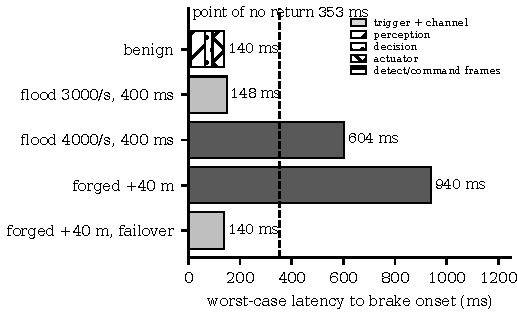
\includegraphics[width=\columnwidth]{fig_bound.pdf}
\caption{Worst-case bound for 60\,km/h, obstacle at 24\,m, CPU load 0.3. The benign bound (140\,ms) is split into its components; the dashed line is the exact point of no return (353\,ms). A flood of 3000 frames/s is proven safe, a flood of 4000 frames/s is not, and radar failover returns a forged distance to the benign bound.}
\label{fig:bound}
\end{figure}

\textbf{Soundness.} Across 9 attack families $\times$ 720 samples $\times$ 2 perception policies the bound was never exceeded (0 of 12{,}960 runs), and no simulated collision was ever labelled proven safe. With the defences, 31{,}200 further runs and 260 adversarial searches (5 configurations $\times$ 13 variants $\times$ 4 scenarios, 200 evaluations each) found no counter-example; the first campaign of 90 searches likewise found none after the repairs below. When the ECU timings were scaled from $0.5\times$ to $2\times$, 36{,}000 more runs also found none.

\textbf{What the search found.} An earlier version was violated in 1 of 27 searches: a flood that ends just before the obstacle appears can leave a queue of about 550 frames that is still draining. Two earlier flood versions were also wrong (queue backlog ignored; flood started before the obstacle). A fourth flaw, in the authentication case, was found while the watchdog was added: the watchdog's start time must not precede the appearance of the obstacle. All are fixed and covered by regression tests. We view this as the main evidence that the adversarial check is worth its cost.

\textbf{Tightness.} The median bound is 1.5--2.1$\times$ the observed latency (95th percentile 2--10$\times$, largest for spoofing families), since it stacks worst-case compute times and uses the critical instant. Consequently about 31\% of tight scenarios have a point of no return below even the benign bound (140\,ms in the headline case), and nothing can be certified for them. For the five families that failover handles, 68.5\% of sampled attacks are proven safe and 31.5\% are unknown; for the same attacks the simulation shows 0\% hazards. For floods, 30.3\% are proven safe, 26.7\% hazardous and 43.1\% unknown.

\textbf{Headline.} In the scenario of Fig.~\ref{fig:bound}, a flood starting at the obstacle is proven safe up to 400\,ms at $\le$3000 frames/s, up to 184\,ms at 4000 frames/s and up to 122\,ms at 6000 frames/s.

\subsection{Q3: what the defences close and what remains}
\begin{figure}[t]
\centering
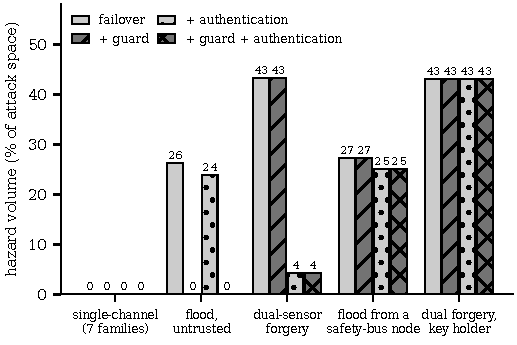
\includegraphics[width=\columnwidth]{fig_defence.pdf}
\caption{Hazard volume by attack variant and defence configuration (600 sampled attacks per bar, each in its own freshly drawn scenario; Wilson interval for the 4.3\% bars: [3.0, 6.3]). Failover is present in every configuration.}
\label{fig:defence}
\end{figure}

Fig.~\ref{fig:defence} shows the result. \textbf{Failover} removes every hazard that needs only the primary channel: masquerade 44.9\% $\rightarrow$ 0.0\% (95\% interval [0.0, 0.5]), gateway delay 25.3\% $\rightarrow$ 0\%, suppression 3.9\% $\rightarrow$ 0\%, jitter 2.6\% $\rightarrow$ 0\% (720 sampled attacks per family). An adaptive attacker finds a hazard against the unprotected chain in 6 of 6 scenarios and in 0 of 6 once failover is on. Failover does \emph{not} help against floods or a dual-sensor attacker (47.8\% $\rightarrow$ 47.5\%). \textbf{The guard} removes floods from the untrusted segment (26.2\% $\rightarrow$ 0.0\%) and costs nothing in latency. \textbf{Authentication with the watchdog} reduces a dual-sensor forgery to 4.3\% [3.0, 6.3] (600 distinct scenarios), at a mean cost of 1.0\,ms. The remaining 4.3\% consists of scenarios whose point of no return is shorter than the time the watchdog needs to notice silence (about 35\,ms) plus the chain.

\textbf{What remains.} With every defence on, two variants stay open: a flood from a node already on the safety bus (25.0\%; adaptive search succeeds in 5 of 6 scenarios) and forging attackers that hold the key (43.0\%; 6 of 6). Authentication moves the trust to key management and the guard moves it to network architecture; neither is general. Fig.~\ref{fig:defence} is stable under changes of the assumptions: the ranking of defences and the list of open variants did not change when braking strength was varied from 0.54\,g (the CARLA-like value) to 0.9\,g, nor when ECU timings changed (at $2\times$ slower ECUs, benign scenarios themselves start to fail: 11 of 40). \emph{Absolute} percentages do depend on these assumptions and should not be quoted as real-world rates.

\textbf{Costs we measured.} Redundant OR-voting trades an integrity hole for an availability hole: a radar forged to report a near obstacle triggers unwanted braking in 100 of 100 trials with failover and 0 of 100 without it. Authentication closes that hole (0 of 100) but opens the mirror one: corrupting both channels now makes the watchdog brake with nothing in the way (0 $\rightarrow$ 100 of 100). Fail-safe behaviour trades integrity for availability; it is a design choice, not a free improvement. A negative result: a variant that brakes whenever the channels disagree by more than 3\,m was identical to plain failover, because the channels disagree only once the attack already hides the real distance.

\textbf{Real MAC.} Replacing the idealised check by a truncated HMAC-SHA256 with a counter changes the picture little: 10{,}631 forged frames were accepted at the theoretical rates (4-bit: 6.26\% against 6.25\%; 8-bit: 0.395\% against 0.391\%; 16- and 24-bit: none), and the 24-bit real tag gives the same trigger source and outcome as the idealised mode in 800 of 800 attacked runs. A side effect that the idealised mode hid: the freshness counter rejects genuine frames that an attack merely reorders (at least one in 200 of 200 jitter-injection runs).

\subsection{Real data, a physics engine and an embedded port}
Table~\ref{tab:real} summarises the checks; the following paragraphs give what each supports and what it does not.

\begin{table}[t]
\caption{Checks against data outside the emulator.}
\label{tab:real}
\centering
\footnotesize
\begin{tabular}{@{}p{0.2\columnwidth}p{0.73\columnwidth}@{}}
\toprule
Source & Result \\
\midrule
ROAD, masquerade (13 captures) & signal rules fused: 0.54 detected within 100\,ms; frame-rate IDS: 0.00; authentication + watchdog: 13/13, median 30\,ms at $k{=}3$, about 6 false triggers/h on the road \\
HCRL, DoS (300 bursts) & flood bound \emph{not} validated; bursts last 4.4--4.9\,s; silence noticed in 300/300, median 127\,ms \\
HCRL, attack-free (253\,s held out) & 0 false watchdog events (95\% upper bound 43/h) \\
CARLA, braking plant & point of no return: 11\,ms error with fitted parameters, 506\,ms with defaults \\
Embedded C port & 138/138 cases identical on two compilers; 528\,B of code (host build) \\
\bottomrule
\end{tabular}
\end{table}

\textbf{ROAD (one vehicle).} Signal rules learned from normal driving only, with zero false alarms on held-out data, catch real forged speed and coolant signals within milliseconds, but miss in-range forgeries such as reverse-light flags (0 of 6), and a per-ID rate IDS cannot be tuned to a usable false-alarm rate on real traffic (about 409 events/h at its least sensitive setting). Replacing a genuine frame keeps the frame rate, so rate-based detectors have no signal by construction. We replayed authentication plus a silence watchdog: with the labelled frames rejected (idealised authentication), the attacked ID falls silent and all 13 captures are detected, median 30\,ms at $k=3$ (Fig.~\ref{fig:road}). The detection follows from the assumption; what the data adds is the timing and the price: 41.5 false triggers per hour over all learned IDs (22/h and about 6/h on the real road if only the sensing IDs are watched), which the emulator hid.

\begin{figure}[t]
\centering
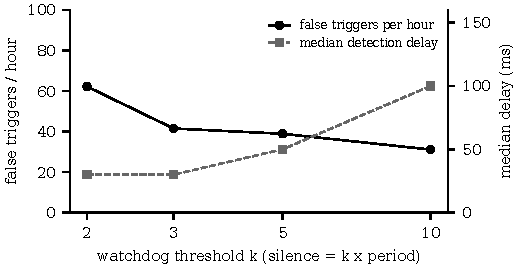
\includegraphics[width=\columnwidth]{fig_road.pdf}
\caption{ROAD: the watchdog threshold trades false triggers against detection delay (13 masquerade captures; 2{,}778\,s of held-out normal driving).}
\label{fig:road}
\end{figure}

\textbf{HCRL (second vehicle).} On the attack-free file (988{,}871 frames, 27 IDs) the watchdog learned on the first half raised no false event on the second half at any of $k\in\{2,3,5,10\}$; 253\,s is short, so the 95\% upper bound is 43 per hour. The 300 real DoS bursts (ID 0x000, 4.56\,s median) silence the 10\,ms messages for 1.3\,s median per ID, about thirteen times a 100\,ms deadline, and the watchdog noticed all 300 bursts. This capture does \emph{not} validate the flood bound: the logger kept about 13\% of the documented flood rate, so a silence may be starvation or logger loss. Using the response-time analysis with a periodic 0.3\,ms flood, the longest silence exceeds the bound for 6 of 26 IDs, so a periodic-flood model does not fit. With a saturating flood, which is the backlog model our bound uses, 1 of 26 IDs exceeds it (0.3\,s over a 5.1\,s bound). The data are consistent with the backlog model, but equally with logger loss. The injection captures show that the spoofed ID's genuine stream is not silenced selectively (4.7\% of gaps over the threshold for the RPM ID against 5.3\% for other IDs), but every ID is degraded and we draw no false-trigger rate from the attack files.

\begin{figure}[t]
\centering
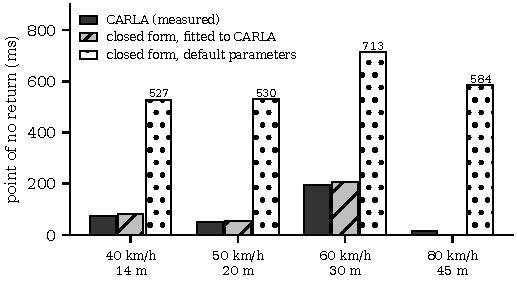
\includegraphics[width=\columnwidth]{fig_carla.pdf}
\caption{CARLA's point of no return against the closed form, for four scenarios (two further scenarios are unavoidable collisions in both). With two fitted parameters the closed form follows CARLA to 11\,ms on average; with its default parameters it is off by 506\,ms. The 80\,km/h bar for the fitted form is $-4$\,ms, plotted as zero.}
\label{fig:carla}
\end{figure}

\textbf{CARLA.} Our first runs were not validation: the vehicle was teleported to speed, its wheels started at rest, and fitted deceleration was 25--60\,m/s$^2$. Starting the car under throttle control gave realistic 5--8\,m/s$^2$. In the full run (Fig.~\ref{fig:carla}) the model structure (hold speed, short ramp, constant deceleration) reproduces CARLA's point of no return to about 10\,ms after two parameters are fitted, but the emulator's defaults (7.85\,m/s$^2$, 50\,ms) are optimistic for this vehicle (CARLA's Model~3 brakes at 4.7--5.5\,m/s$^2$). This is why we vary braking strength in the evaluation.

\textbf{Embedded port.} The perception-side logic (trigger, failover, authentication hook, watchdog) is implemented in portable C99 with integer arithmetic, no allocation and no loops. All 138 test cases (120 recorded from emulator runs, 18 hand-built edge cases) agree exactly with an integer reference on two compilers (528\,B and 490\,B of code on host builds). It has not been run on a microcontroller; the figures are indicative only.

\subsection{LLM-assisted components}
Earlier stages of this work used a language model to turn natural-language requirements into timing specifications and to propose monitor rules. We report them briefly, as results rather than as selling points. Deadline extraction is essentially solved on our 120 author-written requirements (0.99 correct against 0.86 for a regular-expression baseline), but asked to list vehicle-signal paths from memory, the model invented 172 of 185 (93\%); retrieval from the real signal catalogue brings identifier F1 to 0.88 with no invalid path. For rule synthesis, random proposals plus a deterministic verifier reached the same hardened monitor as the language model (a cross-check between the two distance sensors) at the same cost; the verifier, not the model, does the work. The model could not help against the dual-sensor attacker (about 43\%), which no rule over these signals can detect.

\section{Discussion and Limitations}
\label{sec:limits}
\textbf{An error we found in our own method.} Until we corrected it, our experiments sampled attacks over only five or six base scenarios, each reused for many sampled attacks. One unusually tight scenario then moved an estimate by one sixth, and the dual-sensor residual after authentication looked like 1--2\%. With one fresh scenario per sampled attack it is 4.3\% [3.0, 6.3]; three seeds of 300 gave 3.3--5.3\%. The conclusion that authentication leaves a small but real residual survived, the number did not. We recommend fresh scenarios per sample for any hazard-volume estimate.

\textbf{Limits of the evidence.}
\begin{itemize}
\item \emph{Emulation.} ECU compute times, bus load and the 0.5\,ms verification time are assumptions. The sensitivity checks show the qualitative ranking is stable, not that the absolute numbers are right. Nothing here certifies a real vehicle.
\item \emph{Key management is not modelled.} A key holder defeats the design (43\%). This is a boundary of the claim, not a finding about any real key scheme.
\item \emph{One safety function, one vehicle model in CARLA, one road.} The braking plant is a constant-deceleration model; CARLA's braking depends on speed.
\item \emph{The bound is conservative} (median 1.5--2.1$\times$), so many instances are ``unknown'', and it is valid only under the assumptions in Section~IV.
\item \emph{Real attacks.} ROAD contains masquerade but no braking and no consistent dual-sensor attacker; the HCRL captures are lossy; authentication in the replays is idealised. The flood bound has not been validated on lossless real data.
\item \emph{Novelty.} The detection deadline is prior work. Our contribution is its application to CAN timing with an attack-aware bound, the defence assessment, and the honest accounting of what holds.
\end{itemize}

\textbf{Ethics.} All experiments use an emulator, simulated CARLA runs and public datasets; no attack was run on a vehicle.

\section{Conclusion}
For a CAN braking chain, protection should be judged by whether it arrives before the point of no return. An attack-aware response-time bound can prove many attack instances harmless for every random draw, survived large-scale simulation and adversarial search, and found real flaws in its own earlier versions. Radar failover, a gateway guard and authentication with a watchdog close most attack classes, but a flood from a node on the safety bus and an attacker holding the key remain open, and a dual-sensor forgery still succeeds in 4.3\% of the attack space. A high F1 score (0.95) coexisted with 63\% protection in time. The real-data checks support the timing behaviour of the watchdog on two vehicles and the structure of the braking model, and they leave the flood bound unvalidated. Future work includes a hardware test bed, lossless flood captures, a key-management model and a second safety function.

\textbf{Artifact.} An anonymised copy of the code, scripts, logs and the cloud-reproduction results is available to reviewers at [anonymous repository link to be inserted].

\begin{thebibliography}{99}
\bibitem{stachowski2019} S.~Stachowski, R.~Gaynier, and D.~LeBlanc, ``An assessment method for automotive intrusion detection system performance,'' NHTSA, Rep. DOT HS 812 708, 2019.
\bibitem{akowuah2021} F.~Akowuah and F.~Kong, ``Real-time adaptive sensor attack detection in autonomous cyber-physical systems,'' in \emph{Proc. IEEE Real-Time and Embedded Technology and Applications Symposium (RTAS)}, 2021.
\bibitem{akowuah2023} F.~Akowuah, K.~Fletcher, and F.~Kong, ``Variable window and deadline-aware sensor attack detector for automotive CPS,'' 2023.
\bibitem{zhang2020} L.~Zhang, X.~Chen, F.~Kong, and A.~A.~C\'ardenas, ``Real-time attack-recovery for cyber-physical systems using linear approximations,'' in \emph{Proc. IEEE Real-Time Systems Symposium (RTSS)}, 2020.
\bibitem{davis2007} R.~I.~Davis, A.~Burns, R.~J.~Bril, and J.~J.~Lukkien, ``Controller Area Network (CAN) schedulability analysis: Refuted, revisited and revised,'' \emph{Real-Time Systems}, vol.~35, no.~3, pp.~239--272, 2007.
\bibitem{berdich2024} A.~Berdich and B.~Groza, ``Cyberattacks on adaptive cruise controls and emergency braking systems: Adversary models, impact assessment, and countermeasures,'' \emph{IEEE Trans. Reliability}, vol.~73, no.~2, 2024.
\bibitem{zhangthesis} Zhang, ``Safety/security co-design for automotive CAN buses,'' Dissertation, TU Chemnitz, 2024.
\bibitem{ponr2026} ``Beyond time to collision: The point of no return as a reliable safety indicator in rear-end vehicle conflicts,'' \emph{Applied Sciences}, vol.~16, no.~8, 2026.
\bibitem{road} Verma \emph{et al.}, ``ROAD: The Real ORNL Automotive Dynamometer CAN intrusion dataset,'' Oak Ridge National Laboratory, Zenodo record 10462796 (CC-BY 4.0).
\bibitem{hcrl} H.~M.~Song, J.~Woo, and H.~K.~Kim, ``In-vehicle network intrusion detection using deep convolutional neural network,'' \emph{Vehicular Communications}, vol.~21, p.~100198, 2020.
\bibitem{carla} A.~Dosovitskiy, G.~Ros, F.~Codevilla, A.~L\'opez, and V.~Koltun, ``CARLA: An open urban driving simulator,'' in \emph{Proc. Conf. Robot Learning (CoRL)}, 2017.
\bibitem{secoc} AUTOSAR, ``Specification of Secure Onboard Communication,'' AUTOSAR Classic Platform.
\end{thebibliography}

\end{document}
